\chapter{功能安全和信息安全性质}

\section{Safety Property}
Safety Property描述了协议的功能安全性质,在使用sbid工具进行协议建模时,用于对模型进行安全性质规约,用于模型检测的过程中发现伪反例后,通过归纳不变式去除伪反例,从而对模型进行精化。在[协议 > 概览]下,点击小工具栏上的[Safety property]按钮,即可创建新的safety Property的类图,如图\ref{create_safety}所示。
\begin{figure}[h]
	\centering
	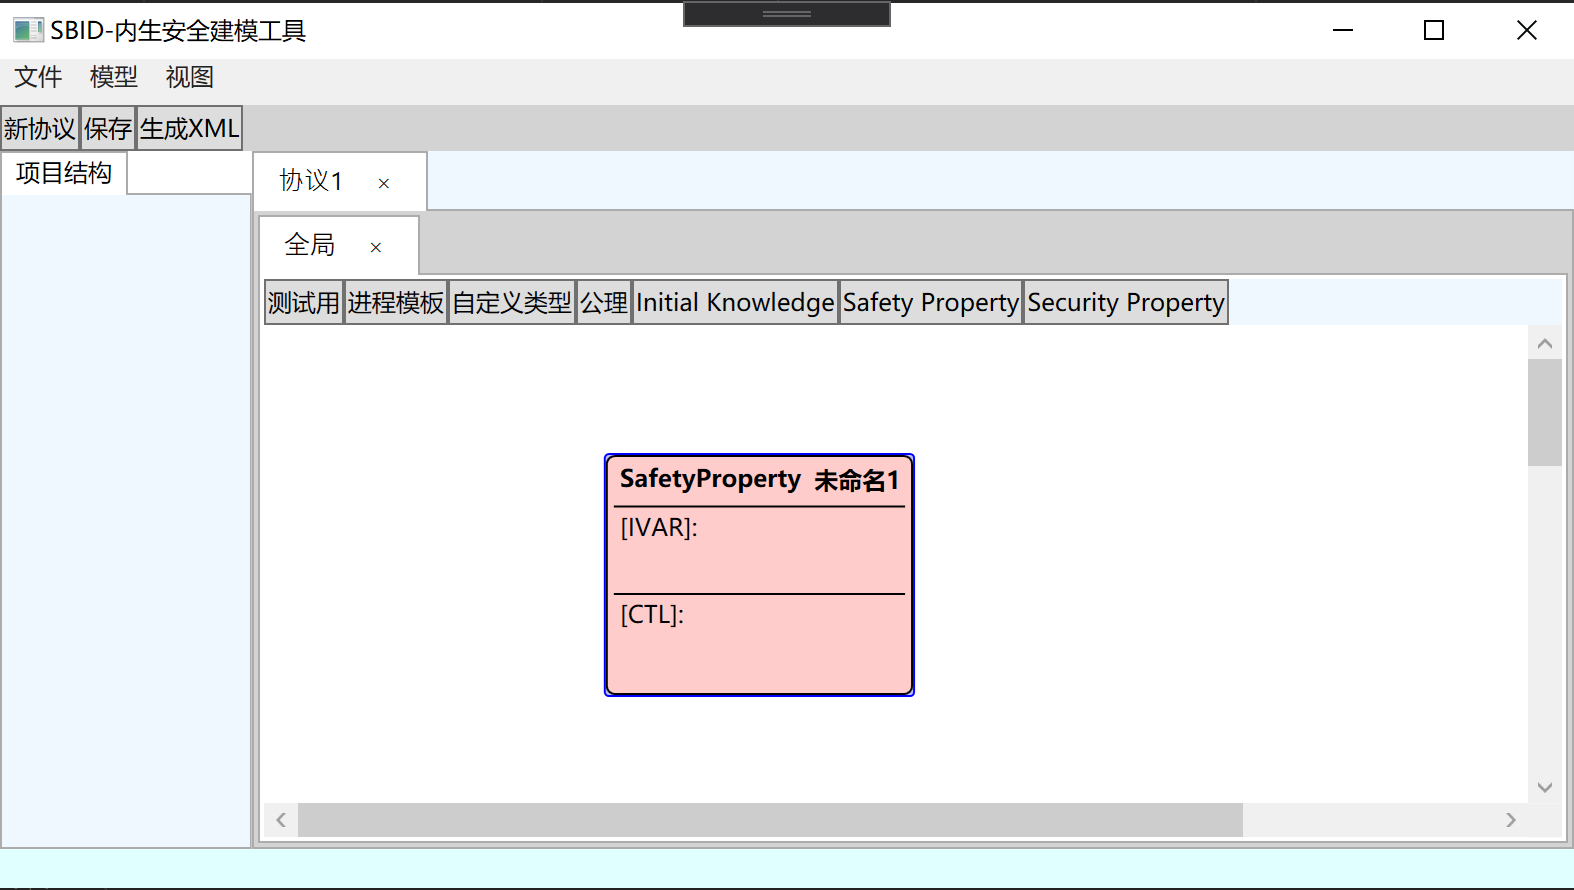
\includegraphics[width=12cm,height=6.75cm]{imgs/create_safety.png}
	\caption{新创建的safety property}
	\label{create_safety}
\end{figure}
\par
在sbid工具中,支持用户对Invariants(不变性)和CTL(Computation Tree Logic)进行描述。
\par
在Safety Property的类图上右键,呼出右键菜单,点击[编辑],即可打开在Safety Property的编辑窗体,如图\ref{safety_edit_window}所示。
\begin{figure}[h]
	\centering
	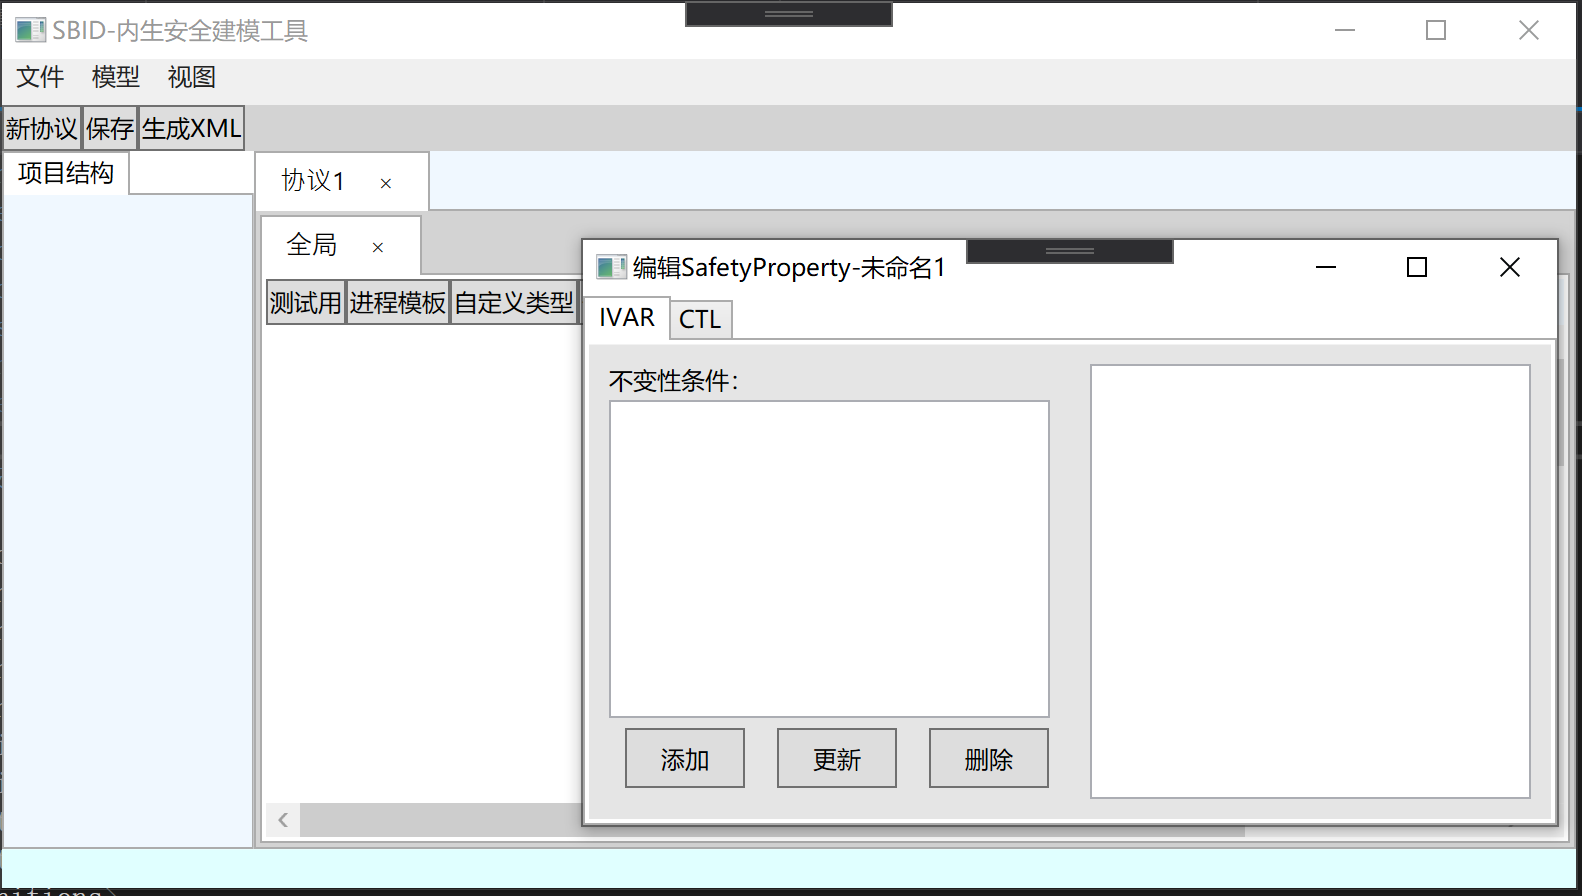
\includegraphics[width=12cm,height=6.75cm]{imgs/safety_edit_window.png}
	\caption{Safety Property的编辑窗体}
	\label{safety_edit_window}
\end{figure}
\par
\subsection{Invariants}
\par
Safety Property的Invariants用于定义模型的不变性条件。打开Safety Property的编辑窗口,选择[IVAR]选项卡,可对Invariants进行添加、修改和删除,如图\ref{safety_edit_invariants}所示。
\begin{figure}[h]
	\centering
	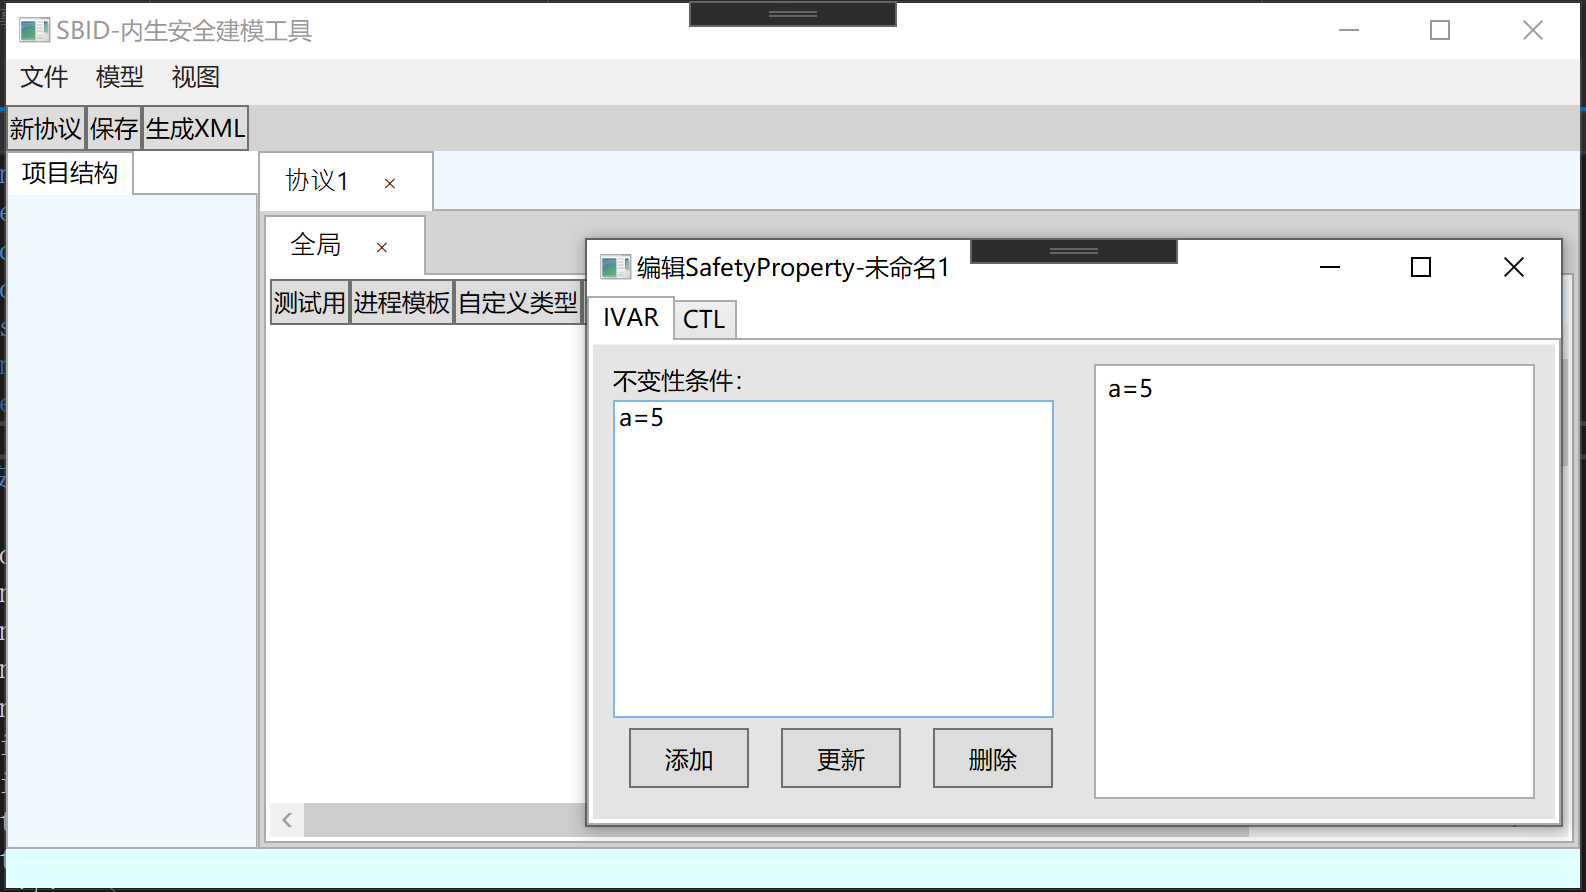
\includegraphics[width=12cm,height=6.75cm]{imgs/safety_edit_invariants.png}
	\caption{编辑Invariants性质}
	\label{safety_edit_invariants}
\end{figure}
\subsection{CTL}
\par
Safety Property的CTL用于定义模型中的计算树逻辑。打开Safety Property的编辑窗口,选择 [CTL]选项卡,可对CTL性质进行添加、修改和删除,如图\ref{safety_edit_CTL}所示。
\begin{figure}[h]
	\centering
	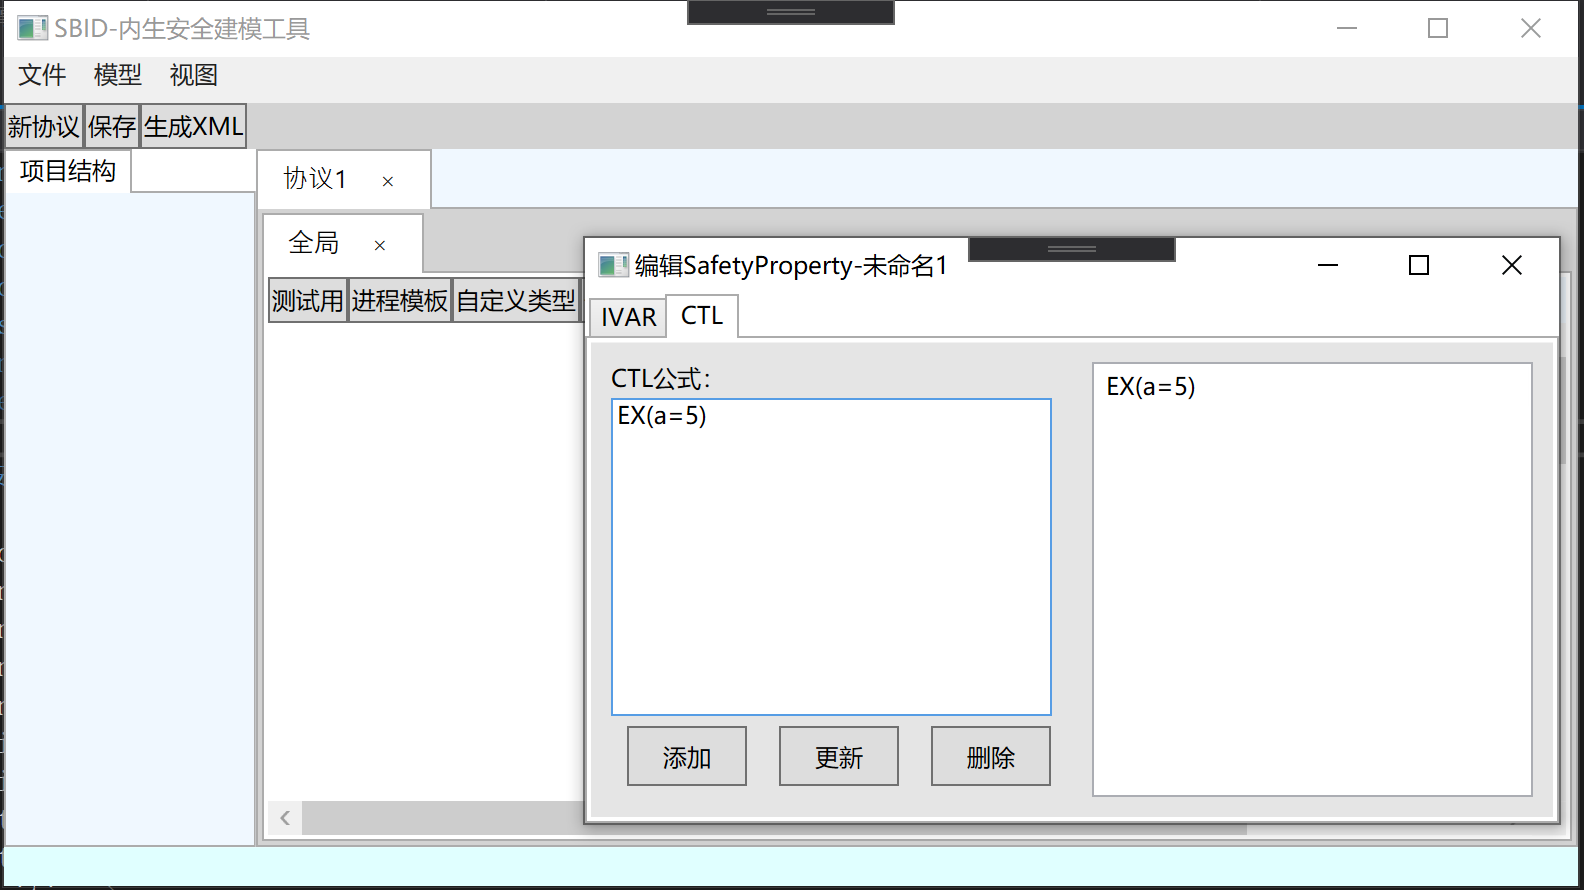
\includegraphics[width=12cm,height=6.75cm]{imgs/safety_edit_CTL.png}
	\caption{编辑的CTL性质}
	\label{safety_edit_CTL}
\end{figure}

\section{Security Property}
Security Property描述了协议进程间的信息安全性质,在使用sbid工具进行协议建模时,对协议进行认证性和机密性描述是非常重要的。在[协议 > 概览]下,点击小工具栏上的[Security Property]按钮,即可创建新的security Property的类图,如图\ref{create_security}所示。
\begin{figure}[h]
	\centering
	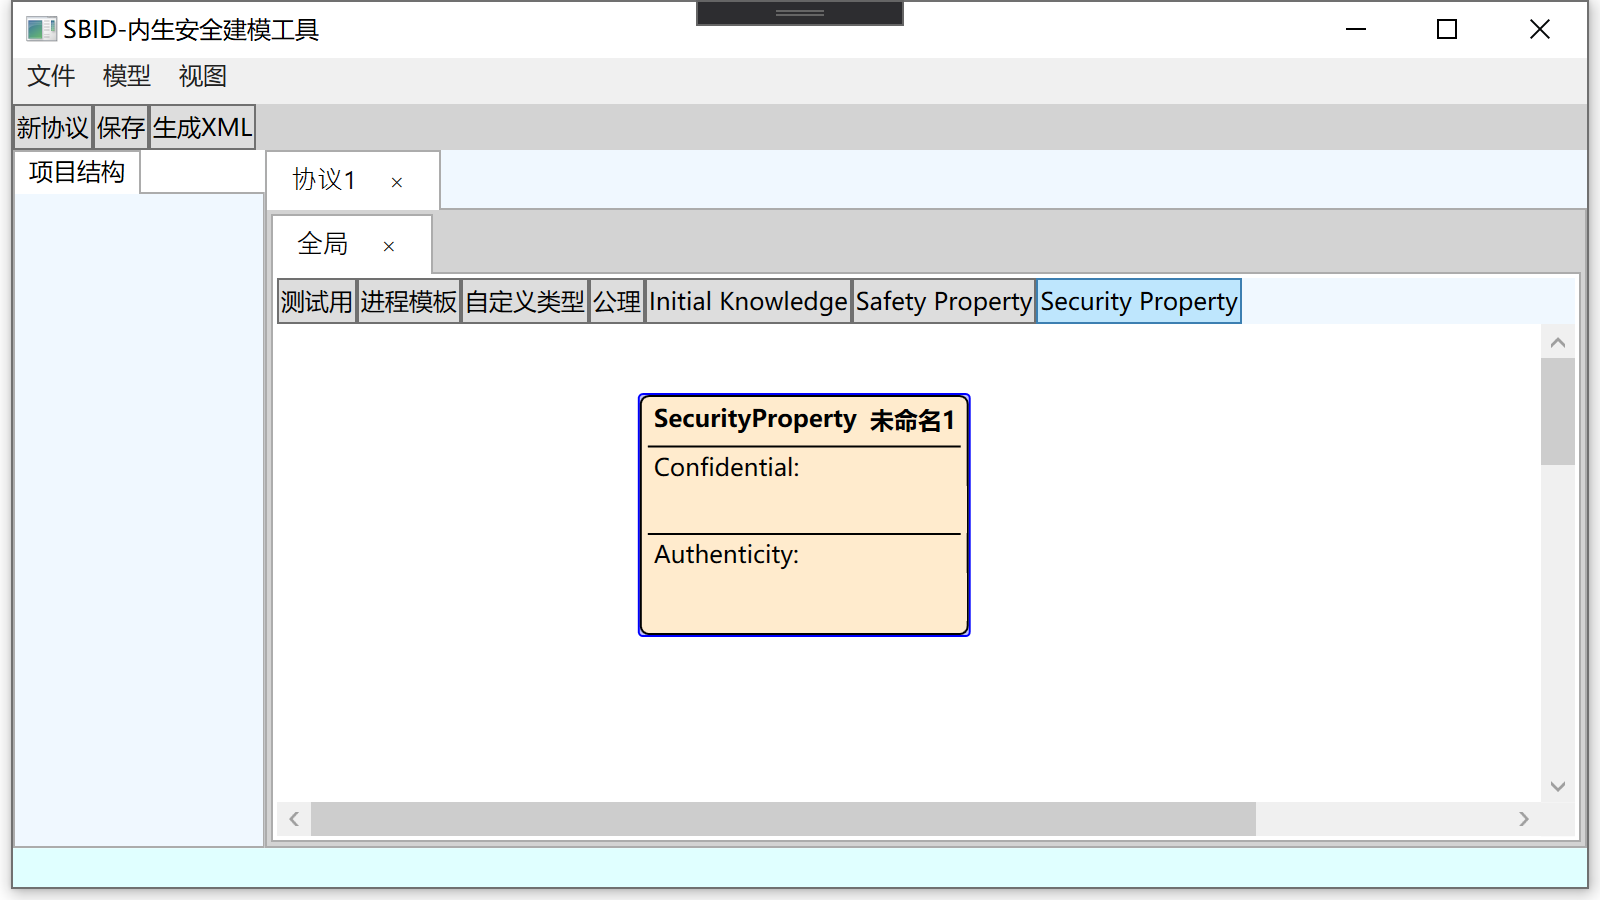
\includegraphics[width=12cm,height=6.75cm]{imgs/create_security.png}
	\caption{新创建的security property}
	\label{create_security}
\end{figure}
\par
在sbid工具中,支持用户对Confidential和Authenticity两类信息安全性质进行描述。
\par
在Security Property的类图上右键,呼出右键菜单,点击[编辑],即可打开在Security Property的编辑窗体,如图\ref{security_edit_window}所示。
\begin{figure}[h]
	\centering
	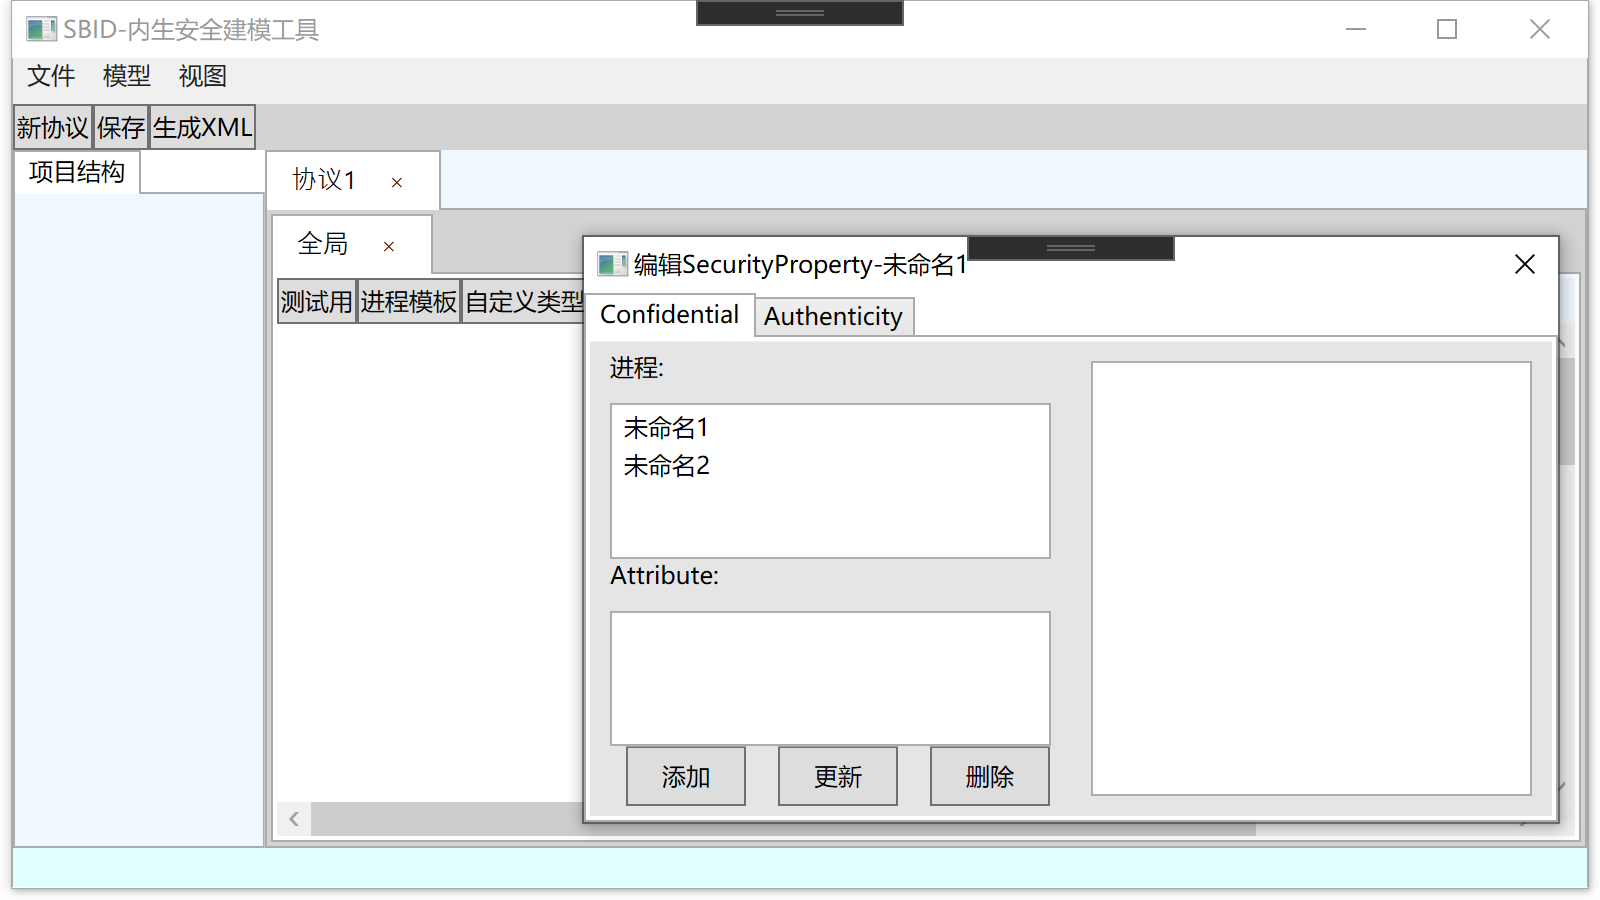
\includegraphics[width=12cm,height=6.75cm]{imgs/security_edit_window.png}
	\caption{Security Property的编辑窗体}
	\label{security_edit_window}
\end{figure}
\par
\subsection{Security Property的Confidential性质}
Security Property的Confidential用于定义进程属性的机密性,需要选中进程的某个属性。打开Security Property的编辑窗口,选择[Confidential]选项卡,可对Confidential进行添加、修改和删除,如图\ref{security_edit_confidential}所示。
\begin{figure}[h]
	\centering
	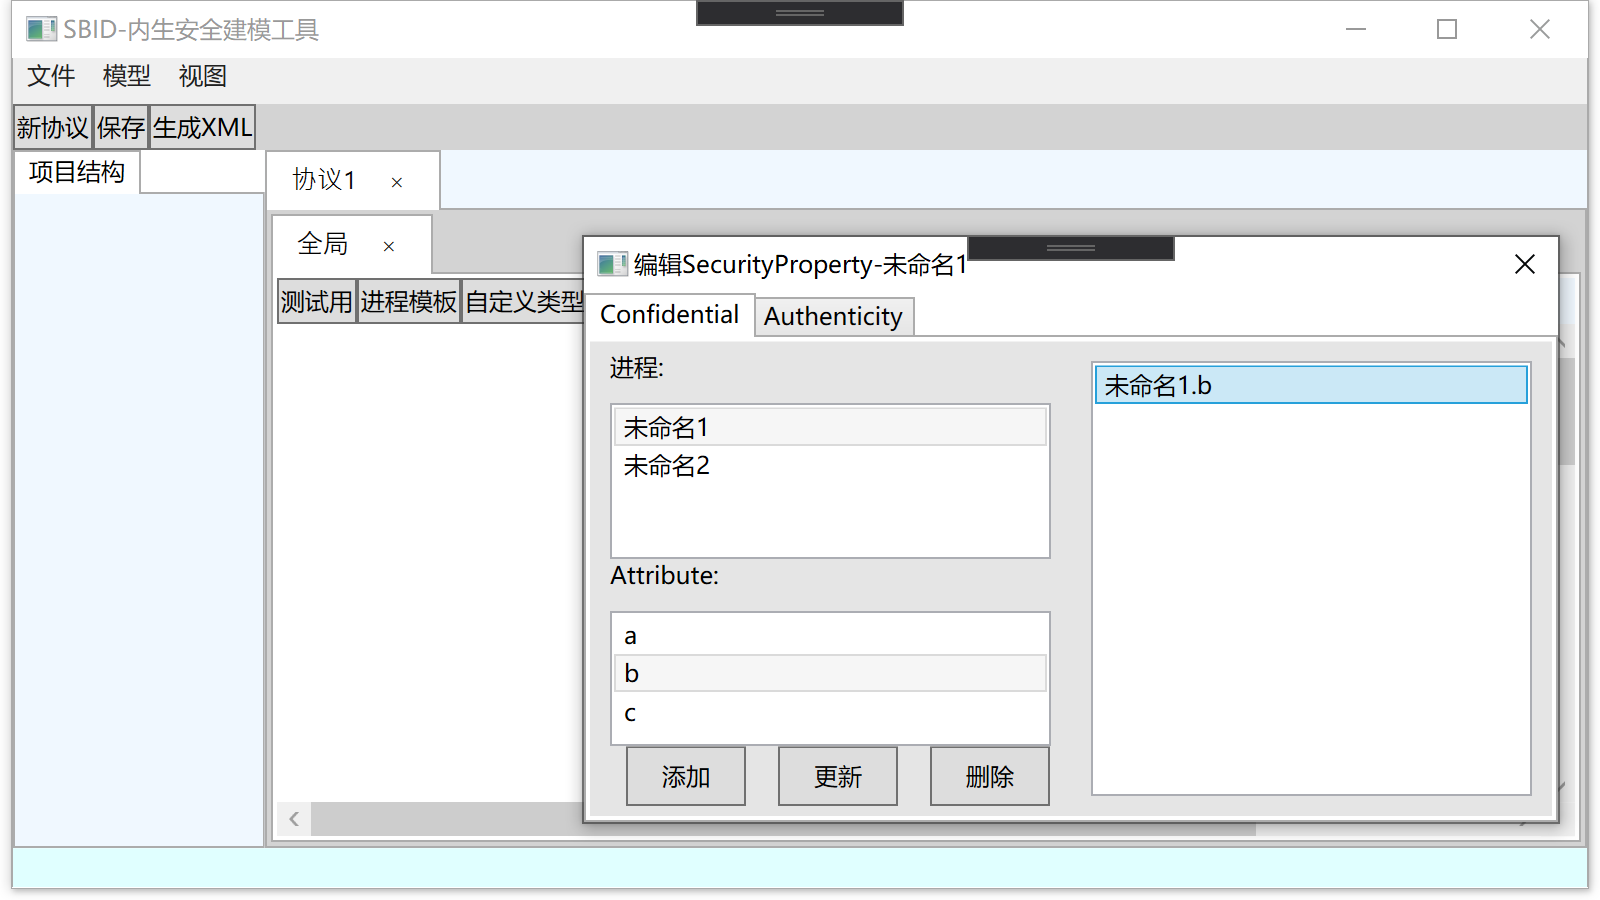
\includegraphics[width=12cm,height=6.75cm]{imgs/security_edit_confidential.png}
	\caption{编辑Confidential性质}
	\label{security_edit_confidential}
\end{figure}
\subsection{Security Property的Authenticity性质}
Security Property的Authenticity用于定义进程状态中属性的认证性,认证性与机密性相比,需要选中两个进程状态的属性。打开Security Property的编辑窗口,选择 [Authenticity]选项卡,可对Authenticity性质进行添加、修改和删除,如图\ref{security_edit_authenticity}所示。
\begin{figure}[h]
	\centering
	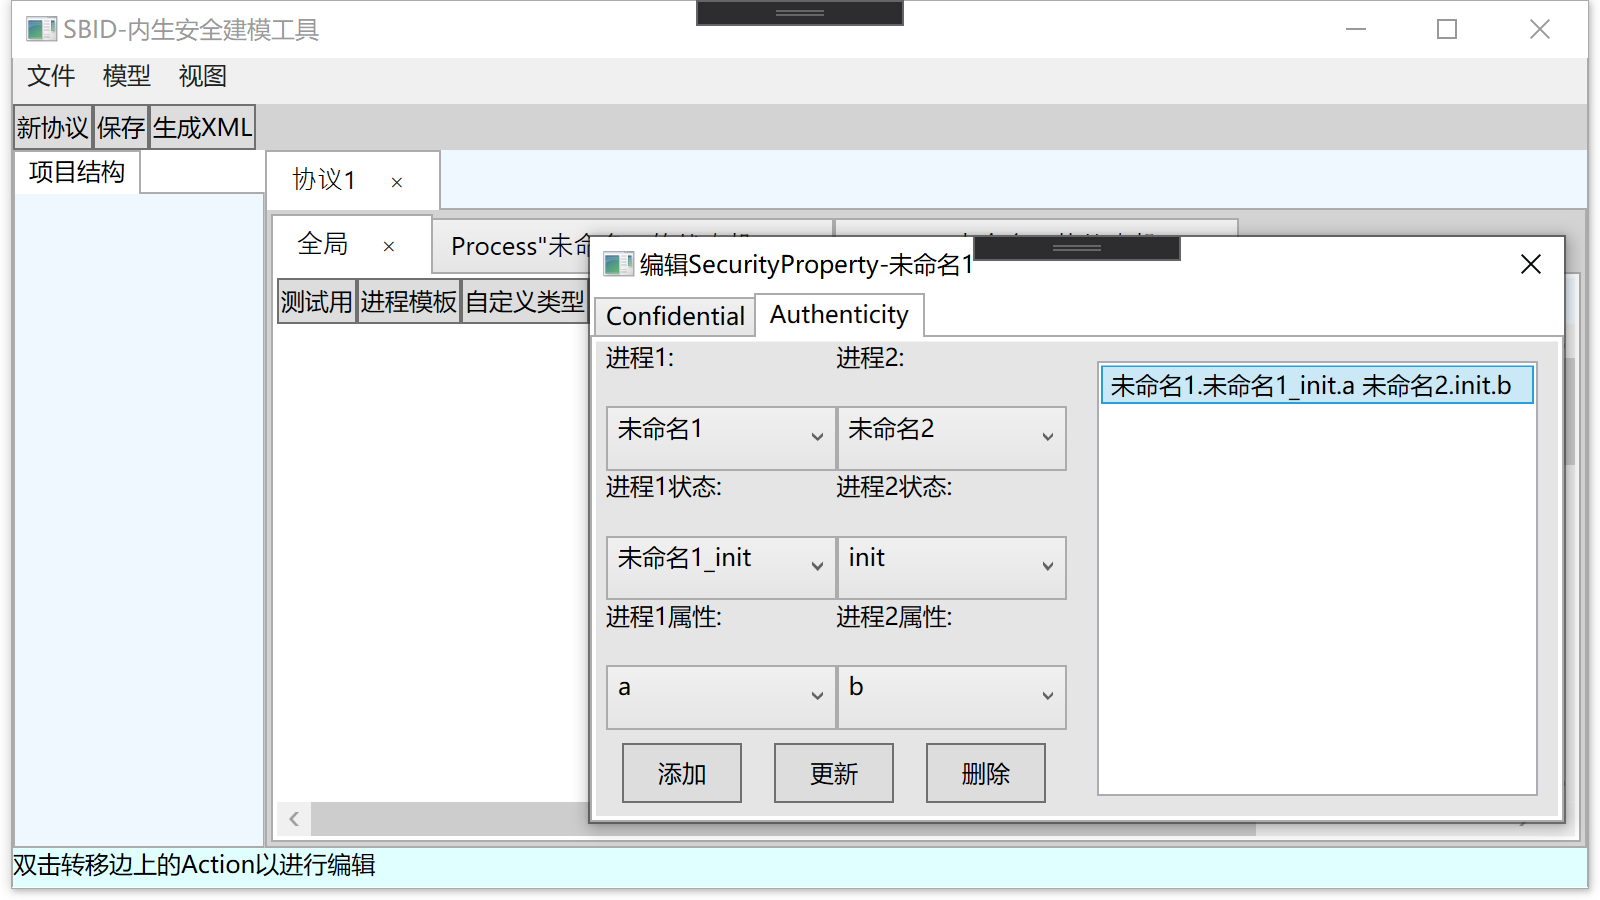
\includegraphics[width=12cm,height=6.75cm]{imgs/security_edit_authenticity.png}
	\caption{编辑的Authenticity性质}
	\label{security_edit_authenticity}
\end{figure}
\par
需要注意,因为Authenticity性质需要使用进程模板状态机上的状态,所以对要使用的进程模板必须先创建状态机,才能在Authenticity性质编辑时选中。